\documentclass[a4paper,twoside,12pt]{report}
% Richard Klein (2020,2021)

% Include Packages
%\usepackage[a4paper,inner=3.5cm,outer=2.5cm,top=2.5cm,bottom=2.5cm]{geometry}  % Set page margins
\usepackage{fullpage}
\usepackage{float}                  % Allows 'Here and Only Here' [H] for Floats
\usepackage{url}                    % \url{} command
\usepackage{charter}                  % Set font to Times
\usepackage{graphicx}               % \includegraphics
\usepackage{subfigure}              % Allow subfigures
\usepackage{amsmath}
\usepackage{amssymb}
\usepackage{amsthm}
\usepackage{booktabs}
\usepackage{parskip}
\usepackage{longtable}
\usepackage[all]{nowidow}
\setnoclub[2]
\setnowidow[2]

% Referencing
% Provides \Vref and \vref to indicate where a reference is.
\usepackage{varioref} 
% Hyperlinks references
\usepackage[bookmarks=true,bookmarksopen=true]{hyperref} 
% Provides \Cref, \cref, \Vref, \vref to include the type of reference: fig/eqn/tbl
\usepackage{cleveref} 
% Setup Hyperref
\hypersetup{
  colorlinks   = true,              %Colours links instead of ugly boxes
  urlcolor     = blue,              %Colour for external hyperlinks
  linkcolor    = blue,              %Colour of internal links
  citecolor    = blue                %Colour of citations
}
% Names for Clever Ref
\crefname{table}{table}{tables}
\Crefname{table}{Table}{Tables}
\crefname{figure}{figure}{figures}
\Crefname{figure}{Figure}{Figures}
\crefname{equation}{equation}{equations}
\Crefname{equation}{Equation}{Equations}

% Wits Citation Style
\usepackage{natbib} % Force natbib.sty to put citation labels in the reference list
\makeatletter
\renewcommand\NAT@biblabel[1]{\def\citeauthoryear##1##2{##1 ##2}[#1]\hfill}
\renewcommand\NAT@bibsetup[1]{%
  \setlength{\itemsep}{\bibsep}\setlength{\parsep}{\z@}}
\def\@lbibitem[#1]#2{%
  \if\relax\@extra@b@citeb\relax\else
    \@ifundefined{br@#2\@extra@b@citeb}{}{%
     \@namedef{br@#2}{\@nameuse{br@#2\@extra@b@citeb}}}\fi
   \@ifundefined{b@#2\@extra@b@citeb}{\def\NAT@num{}}{\NAT@parse{#2}}%
   \item[\hfil\hyper@natanchorstart{#2\@extra@b@citeb}\@biblabel{#1}%
    \hyper@natanchorend]%
    \NAT@ifcmd#1(@)(@)\@nil{#2}}
\makeatother


\bibliographystyle{named-wits}
\bibpunct{[}{]}{;}{a}{}{}  % to get correct punctuation for bibliography
\setlength{\skip\footins}{1.5cm}
\newcommand{\citets}[1]{\citeauthor{#1}'s \citeyearpar{#1}}
\renewcommand\bibname{References}  

\pagestyle{headings}

\pagestyle{plain}
\pagenumbering{roman}

\renewenvironment{abstract}{\ \vfill\begin{center}\textbf{Abstract}\end{center}\addcontentsline{toc}{section}{Abstract}}{\vfill\vfill\newpage}
\newenvironment{declaration}{\ \vfill\begin{center}\textbf{Declaration}\end{center}\addcontentsline{toc}{section}{Declaration}}{\vfill\vfill\newpage}
\newenvironment{acknowledgements}{\ \vfill\begin{center}\textbf{Acknowledgements}\end{center}\addcontentsline{toc}{section}{Acknowledgements}}{\vfill\vfill\newpage}

\begin{document}
\onecolumn
\thispagestyle{empty}

\setcounter{page}{0}

\begin{center}
  \vfill
  {
  \huge \bf \textsc{The Adaptation of an IoT Air Quality Monitoring System for use in Underground Mines}
  \vspace{50pt}\\
  \large School of Computer Science \& Applied Mathematics\\
  \large University of the Witwatersrand\\[20pt]
  \normalsize
  Alexandra Barry\\
  1056862\\[20pt]
  Supervised by Bruce Mellado\\[10pt]
  \today
  }

  \vfill
  \vfill
  
\includegraphics[width=1.5cm]{images/wits}
  \vspace{10pt}\\
  \small{A proposal submitted to the Faculty of Science, University of the Witwatersrand, Johannesburg,
in partial fulfilment of the requirements for the degree of Master of Science}\\
\end{center}
\vfill
\newpage

\pagestyle{plain}
\setcounter{page}{1}

\phantomsection
\begin{declaration}
I, Alexandra May Barry, hereby declare the contents of this research proposal to be my own work.
This proposal is submitted as a requirement for the course 'COMS7060' within of the degree of Master of Science in Robotics at the University of the Witwatersrand.
This work has not been submitted to any other university, or for any other degree.
\end{declaration}

\phantomsection
\begin{abstract}
Air quality monitoring is an important aspect of ensuring safe and healthy living and working environments. Readings and predictions of air quality can assist governing bodies in applying appropriate mitigation steps and policies to reduce air pollution where necessary. The South African Consortium of Air Quality Monitoring (SACAQM) developed a low cost monitoring system, 'AI\_r', that comprises of IoT sensor nodes connected to the cloud. The readings of these are processed with machine learning algorithms to provide accurate real-time predictions. 
\newline \newline
This report examines the practicality of extending the AI\_r system into a mining context and analyzes the methods that can be employed to optimize the wireless communication protocols within the system.
\end{abstract}

\phantomsection
\tableofcontents
\newpage
\phantomsection
\addcontentsline{toc}{section}{List of Figures}
\listoffigures
\newpage
\phantomsection
\addcontentsline{toc}{section}{List of Tables}
\listoftables
\newpage
\pagenumbering{arabic}

\chapter{Introduction}
Air pollution poses a great risk to human health. Millions of lives can be spared by reducing air pollution as it has been shown to increase the risk of lung cancer, heart disease, strokes and other respiratory diseases \citep{WHO_2022}. Having access to air quality measurements allows for the better management and prevention of air pollution. Investments and policies can be implemented to help improve conditions that do not meet regulatory guidelines, such as the WHO Global air quality guidelines (AQG).
\newline

An industry that faces critical air quality issues is the mining industry. Miners are routinely exposed to harmful aerosols. Ventilation systems can be put in place however, to improve these conditions. A large proportion of the energy consumed in mining operations is due to these ventilation systems and thus an air quality monitoring system can be put in place to optimize the cost and safety of operating a mine\citep{Hercus_2022}.
\newline

The South African Consortium of Air Quality Monitoring (SACAQM), in partnership with various other organizations, developed an AI-powered IoT system of air quality monitoring sensors that measure and predict air quality in real time \citep{SACAQM}. This system was developed to make predictions for outdoor locations spanning over wide territories. The system was not designed for use in underground mines as as such, various analyses will need to be made to determine any necessary adaptions to be made to the system.
\newline

While several studies have been conducted on the performance of IoT systems in underground contexts, none is specific to the context of this system and with the system's specific components. This report will investigate what adaptations are required. Chapter 2 details the background and related work that has been conducted around the topics of IoT air quality monitoring and underground radio wave propagation, Chapter 3 outlines the research problem and stipulates the steps required to complete the research and, finally, Chapter 4 provides a schedule for the work to be undertaken.

\chapter{Background and Related Work}

\section{Introduction}
This chapter details the existing project: 'AI\_r' for which this research is an extension of, examines the importance of air quality monitoring and explores related research and similar projects.

\section{Background}
\subsection{Air Quality Monitoring}
 Air pollution has been linked to many health impediments such as heart disease, strokes, lung cancer and both acute and chronic respiratory diseases \citep{WHO_2022}. The World Health Organization (WHO) has created a set of air quality guidelines (AQG) that stipulate the thresholds and limits for air pollutants that are known to create risks to ones health. \cite{WHO_2022} has claimed that in 2019, 99\% of the world's population was living in an environment with air quality below these regulatory guidelines. Policies and investments can be made by governing bodies to mitigate air pollution by supporting better practices in power generation, transportation, industry and waste management.
 \newline \newline
Many harmful aerosols, including: quarts, silica, arsenic, diesel and particulate matter are generated during the mining process and this affects miners both under and above ground\citep{Hercus_2022}. Real-time, accurate air quality measurements are critical to assist in monitoring whether exposure is above regulatory limits. These readings can be used to warn miners or can indicate the need for improved ventilation and mining practices. It is estimated that 50\% of the energy consumed in mining operations is due to the ventilation systems\citep{Hercus_2022}. Integrating air quality measurements into an automated ventilation control system could provide a cost-effective method of ensuring a healthy supply of fresh air to the miners. Operational health and safety in underground mines can be improved substantially by monitoring conditions such as temperature, gas, noise and dust \citep{Sadeghi2022ApplicationsMines}.

\subsection{The SACAQM AI\_r System}
\subsubsection{Purpose}
The AI\_r system was developed as a solution to the high cost and complexity of traditional air quality monitoring stations\citep{SACAQM}. It will supplement the existing national quality monitoring systems by adding hundreds of thousands of additional sensor nodes. The system is comprised of air quality sensors within an IoT network, powered by Artificial Intelligence with the aim of providing accurate prediction and analysis of air quality in real time\citep{SACAQM}.

\subsubsection{System Architecture}
The AI\_r system includes various layers, from the low-level sensor devices to the real-time analysis and predictive modeling of data received. This section will focus on the sensor devices and network layers, as these are the areas of interest for wireless communication optimization. Figure \ref{fig:AQMSystemOverview} shows a high level overview of the full system.

\begin{figure}[ht]
	\centering
	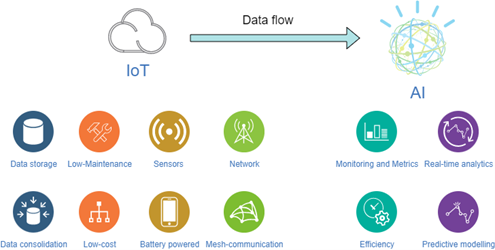
\includegraphics[width=0.5\linewidth]{images/AirQualitySystemOverview.png}
	\caption{AI\_r System High Level Overview}
	\label{fig:AQMSystemOverview}
\end{figure}

The layers of interest can be defined as the following:
\begin{enumerate}
    \item \textbf{The Sensing Layer}: the set of all IoT sensor nodes
    \item \textbf{The Network Layer}: the faciliation of communication across devices, systems and the cloud
\end{enumerate}

An important factor of the Network Layer is reliable and timely transmission of data.
\newline \newline
Figure \ref{fig:NetworkTopology} shows a diagram of the two layers combined. The sensor nodes are connected to one another via a LoRa mesh network and the master nodes connect to the cloud via 4G connections.

\begin{figure}[ht]
	\centering
	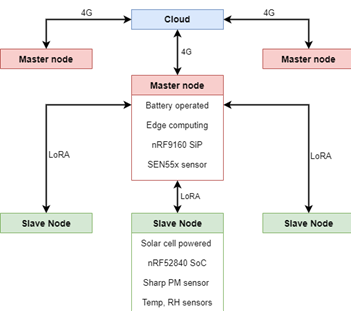
\includegraphics[width=0.4\linewidth]{images/Network_topology_of_AI_r_system_cropped.png}
	\caption{Network Topology of AI\_r System}
	\label{fig:NetworkTopology}
\end{figure}

There are two types of sensor nodes included in the system. The master nodes are based on Nordic Semiconductor nRF5160 SiPs and by default include the following sensor types:
\begin{itemize}
    \item ambient temperature
    \item relative humidity
    \item ambient pressure
    \item SO2
    \item NO
    \item NO2
    \item PM2.5 (high quality)
    \item PM10
\end{itemize}

These measurements require more power and the selection of sensor types per node can be adapted to suit the requirements of the monitoring system. The nodes include an internally housed battery that is expected to power the node for up to one year. These nodes are connected to the cloud via 4G networks.
\newline

The slave sensor nodes are based on the Nordic Semiconductor nRF52840 System on Chip (SoC) and include less accurate PM2.5 sensors. They connect to other master nodes through LoRa (low-power, long range radio communication) and are solar powered.
\newline 

Figure \ref{fig:SensorNodes} shows a computer-generated drawing of one of these sensor nodes (right) and an image of three of the nodes (left).

\begin{figure}[ht]
	\centering
	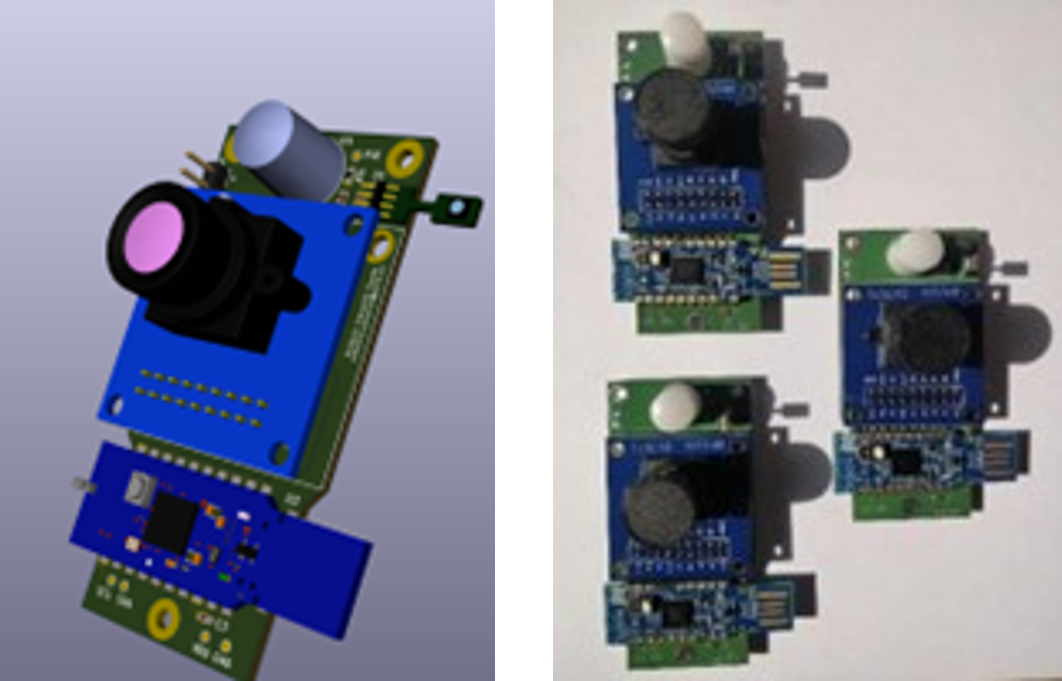
\includegraphics[width=0.5\linewidth]{images/SensorNodes.png}
	\caption{AI\_r Sensor Nodes}
	\label{fig:SensorNodes}
\end{figure}

\subsection{Wireless Communication}
The IoT communication protocol used in the AI\_r system is LoRa, which is a low-power, long range radio communication protocol. LoRa is a physical radio communication technique, based on the spread spectrum modulation technique derived from chirp spread spectrum (CSS)\citep{Semtech_2023}. LoRaWAN is the communication protocol and specifies the system architecture. Together, LoRa and LoRaWAN form a Low Power Wide Area Network (LPWAN) protocol. Figure \ref{fig:LoRaRange} shows an indicational diagram of where LoRa fits in the realm of wireless communication methods.

\begin{figure}[ht]
	\centering
	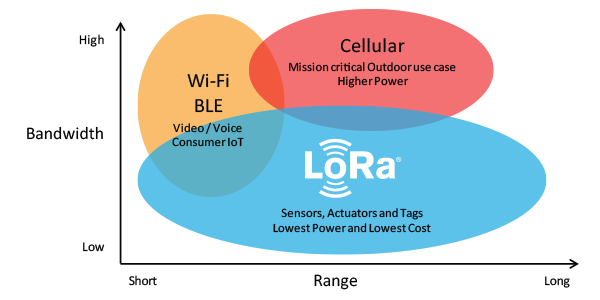
\includegraphics[width=0.5\linewidth]{images/LoRa_Why_Range.png}
	\caption{Diagram of LoRa Range, taken from \cite{Semtech_2023}}
	\label{fig:LoRaRange}
\end{figure}

The AI\_r system uses the sensor nodes in a mesh network. Mesh networks have an arbitrary topology and each node is independent from one another yet connects to the others with multiple redundant nodes. The data intended for a given node is propagated through the nodes until the addressed node is reached. Due to these features, mesh networks are self-configurable and self-healing.
\newline

LoRa communication involves the transmission of packets of data. A full packet is comprised of upchirps and downchirps \citep{Liando2019KnownStudy}. A 'chirp' is a modulated signal that carries data. \Cref{fig:LoRaTransmissionSpectogram} shows a spectrogram of one of these packets of data.

\begin{figure}[ht]
	\centering
	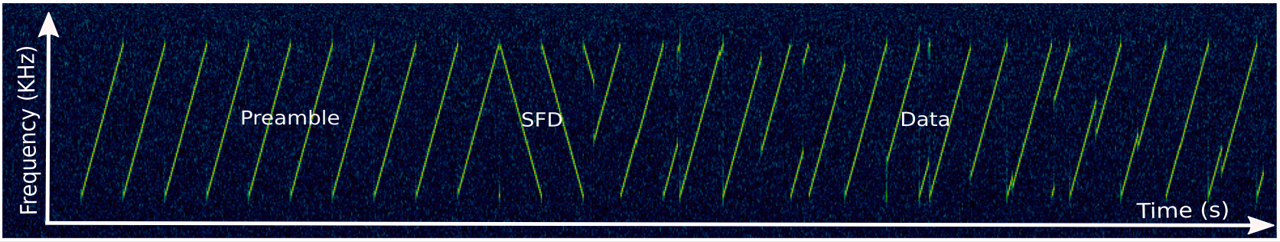
\includegraphics[width=0.8\linewidth]{images/LoRa transmission spectogram.png}
	\caption{Spectogram of LoRa Transmission, taken from \cite{Liando2019KnownStudy}}
	\label{fig:LoRaTransmissionSpectogram}
\end{figure}

The first half of the figure shows the 'upchirps' where the frequency moves from $f_{min}$ (the minimum frequency) to $f_{max}$ (the maximum frequency) and is increasing over time. After this, the 'downchirp' is shown (annotated with 'SDF': Start Frame Delimiter) and goes from $f_{max}$ to $f_{min}$ and finally the modulated chirps follow that contain the data bits.
\newline

\cite{Liando2019KnownStudy} defines four main parameters that can be used to achieve trade-offs between communication distances, data rate and power consumption. These include:
\begin{itemize}
    \item Spreading Factor (SF)
    \item Bandwidth
    \item Transmission Power (Tx Power)
    \item Channel
\end{itemize}

The configurable options of these parameters are shown in Table \ref{tab:LoRaParams} and each will be explained in detail.
\begin{table*}[!htbp]
	\centering
	\caption{LoRa Chipset Configuration Options as Described in \cite{SemtechDatasheet}}
	\label{tab:LoRaParams}
\begin{tabular}{cl}
	\hline
	Parameter & Options\\
	\hline\hline 
	SF & 6, 7, 8, 9, 10, 11, 12 \\ 
	BW (kHz) & 7.8, 10.4, 15.6, 20.8, 31.2, 41.7, 62.5, 125, 250, 500 \\ 
    CR & 4/5, 4/6, 4/7, 4/8 \\ 
	\hline
\end{tabular} 
\end{table*}

\textbf{Spreading Factor (SF)} \newline
The spreading factor affects the angle of the chirps and remains consistent throughout the packet. When a system contains a constant frequency bandwidth, this factor will determine the final data rate \citep{Liando2019KnownStudy}. The highest data rate supported at the time of writing is SF6 which, for successful demodulation, requires the highest signal-to-noise (SNR) ratio. SF12 supports the lowest data rate but correspondingly and for the same transmission power requires the lowest SNR. By incrementing the SF and assuming all other parameters remain constant, the time taken to transmit a chirp is approximately doubled. A longer chirp duration means that receivers have more time to sample the signal power, resulting in a higher SNR.
\newline

\textbf{Bandwidth (BW)} \newline
Bandwidth determines the width of the transmitted signal. The duration of a chirp, $T_{sym}$ can be defined as:
\[ T_{sym} = \frac{2^{SF}}{BW} \citep{LoRaModulation} \] 

Where each chirp consists of $2^{SF}$ number of RF chips carrying SF number of bits. $T_{sym}$ is measured as a chip per Hz of BW.
Therefore, the Bandwidth plays a role in the determination of the chirp duration.
\newline

\textbf{Transmission Power (Tx Pow)} \newline
The increase of transmission power corresponds to a better chance of the signal surviving attenuation caused by the environment however, it directly affects the amount of power drawn.

\section{Related Work}

\subsection{Analyses of LoRa Networks}
Several studies have been conducted to assess and experiment with LoRa configuration to optimize systems with respect to transmission reliability and/or power consumption. \cite{Gkotsiopoulos2021PerformanceReview} performed a review of literature on LoRa-based networks and categorized the main contributing factors to network performance. These categories include:

\begin{itemize}
    \item PHY characteristics \& Phenomena
    \item Deployment features \& Hardware selection
    \item EDs transmission settings \& Features
    \item LoRa MAC protocols
    \item Application requirements \& Policies
\end{itemize}

\Vref{tab:performance-determinants} in the Appendix details some of these contributing factors and the effects of the LoRa parameters on the network performance.
\newline

Another large scale study was conducted by \cite{Liando2019KnownStudy} to experiment with the configurable parameters of LoRa and present what effects these have on the energy consumption and network capacity of the devices. Figure \ref{fig:LoRaTransmissionSpectogram} for example, demonstrates the resulting Packet Reception Ratio (PRR) for devices communicating in line-of-sight and non-line-of-sight environments with variable SFs.

\begin{figure}[ht]
	\centering
	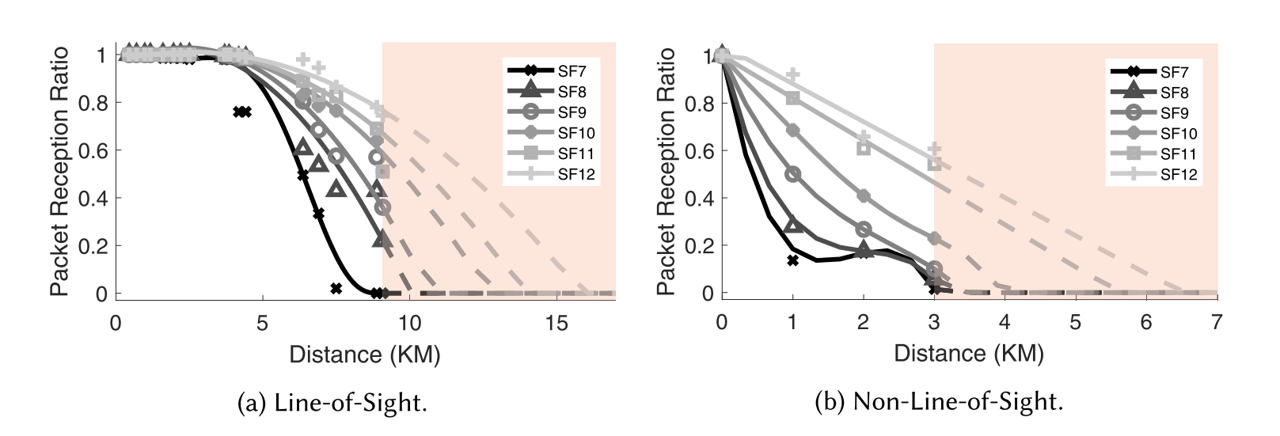
\includegraphics[width=0.8\linewidth]{images/LoRa_propagation_line_of_sight.png}
	\caption{Communication Distances for Varying Spreading Factors in Different Environments, taken from \cite{Liando2019KnownStudy}}
	\label{fig:LoRaTransmissionSpectogram}
\end{figure}


\subsection{IoT Systems in Underground Contexts}
Several studies have too been conducted on IoT networks in underground environments. \cite{Villarim2022EvaluationApplications} conducted tests for transmissions from under to above ground and found that data packets are lost when increasing the depth of the transmitting device. \cite{Ranjan2018DeepSense:Workings} performs real tests to determine radio signal behaviour in metal and non-metal underground mines. \cite{Jo_Khan_2018}, \cite{Zhu2019MonitoringNetwork} and \cite{Ali2022ImprovingSystem} use ZigBee and WiFi based IoT systems to implement monitoring networks while \cite{Ali2022ImprovingSystem} additionally connects the sensors to a control system that activates fans and triggers surface alerts to track the low cost of opening alternative coal.
\newline

Some studies have been conducted to model the radio wave propagation in mines (\citep{MineRadioPredictionModel1}, \citep{MineRadioPredictionModel2},  \citep{MineRadioPredictionModel3}, \citep{Hrovat2014ATunnels}...) and studies such as done by \cite{Emmanuel2019LoRaMines} have used these models to make calculated predictions of network behaviour. \cite{MineRadioPredictionModel3} measured the LoRa PERs in test chambers where the test chambers are designed to simulate the Additive White Gaussian Noise (AWGN) and multipath propagation environments. \cite{Hrovat2014ATunnels} investigated radio propagation in tunnels. Radio propagation in mines can be affected by features of the mine, such as the geometry, mining methods, humidity, wall roughness, temperature, etc. or the parameters of the system, such as: radio signal frequency, position of transceivers etc. The comparison of Bit Error Rate (BER) to SNR can be assessed as a performance determinant\citep{Emmanuel2019LoRaMines}.

\chapter{Research and Methodology}
This section establishes the research question for the project and from which, objectives and deliverables are derived. A methodology for achieving these deliverables is drawn up and the limitations of the project are then discussed.

\section{Introduction and Problem Statement}
The effective management of air quality is critical for governing bodies and individuals to make responsible decisions and ensure healthy living and working conditions. IoT systems have been introduced in this space to replace or complement existing air monitoring systems that are traditionally more expensive and inefficient. 
\newline \newline
The mining sector has particularly concentrated concerns around air quality due to the numerous toxic aerosols both above and under ground. It has been shown that IoT systems can be implemented to assist in improving ventilation or warning miners of unhealthy working conditions. 
\newline \newline
The SACAQM has developed a novel air quality monitoring system that includes several sensor nodes to provide real-time air quality predictions. The system was developed for outdoor use and as such, there may be modifications required to apply this system in a mining context. For example, the system includes solar cells to power the sensor nodes which would not be feasible in underground. The network topology and parameters may not be sufficient to cope with the interference and obstructions in underground tunnels.

\section{Research Question}
The research question for this project is: what modifications should be made to the AI\_r air quality monitoring system to ensure efficient and reliable sensor data transmission from underground mines?

\section{Research Aims and Objectives}

\subsection{Research Aims}
The aims of the research include:
\begin{itemize}
    \item Determining whether the existing features of the AI\_r system are suitable to be used in a mining context or whether modifications to the architecture would need to be made
    \item Determining what set of parameters can be adjusted to optimize the collection of sensor data in terms of power usage and transmission reliability
\end{itemize}

\subsection{Objectives}
The objectives of the research include:
\begin{itemize}
    \item Analyzing existing research on IoT networks in underground contexts to determine whether the AI\_r system will be sufficient
    \item Determining the most appropriate network topology and layout of sensor nodes that would provide reliable data transmissions from an underground mine
    \item Performing tests with the sensor nodes to determine the most efficient network settings
\end{itemize}

\section{Methods and Research Design}
As laid out in the objectives, the project includes both research based and experimental deliverables.

\subsection{Assessment of Architectural Changes to the AI\_r System}
The sensor nodes include a number of sensor types all of which may not be necessary in the calculation of air quality monitoring. An evaluation should be conducted that compares the results of the Machine Learning models and weighted value of each sensor type to the power draw and additional transmission data required. It can then be determined whether any of the sensor types can be omitted from the nodes to reduce the power and transmission requirements.

\subsection{Modeling Underground Interference}
A theoretical analysis should be devised that uses previous studies modeling the nature of radio wave propagation in underground mines to devise a prediction of the most effective layout of sensor nodes as well as the configurable parameters to use in the nodes.

\subsection{Testing for Optimized Network Parameters}
Real life tests should be performed to confirm the predictions made in the theoretical analysis. While access to a real mine is not feasible for this study, a test setup can be created in the University of Witwatersrand mock mine shaft and the results extrapolated upon. The effects of varying the LoRa parameters: SF, BW and Tx Pow will be evaluated to determine the best received power (RSSI) and Signal to Noise Ratio (SNR) results.
\newline
For these tests, a RFM95W LoRa radio will be connected to an Arduino microcontroller to take readings of the RSSI and SNR from a sensor transmitting test readings.


\section{Limitations}
Due to the time constraints and equipment available, limited testing and data collection will be possible.
Access to a real mine for conducting tests will not be possible however, the features of varying mine types will be drawn from research conducted and basic tests can be performed in the Wits mock mine.

\chapter{Schedule of Work}
Table \ref{tab:workScheduleTable} outlines the weekly activities that should be undertaken to fulfil the requirements of this project.
\begin{table*}[!htbp]
	\centering
	\caption{Proposed Schedule of Work for Capstone Project}
	\label{tab:workScheduleTable}
\begin{tabular}{| r | l | c |}
	\hline
	\textbf{Week} & \textbf{Activity} & \textbf{Hours}\\
	\hline\hline 
	July 17 & Gather test equipment and ML results  & 10 \\ 
	24 & Analysis of the ML results for unnecessary sensor inclusions & 20 \\ 
    31 & Devise estimations of the most efficient node layout and parameters & 20 \\ 
    \hline
    Aug 7 & Plan experiments and prepare test data & 20 \\ 
    14 & Perform experiments in the mock mine shaft and record results & 20 \\ 
    21 & Analyze test results and draw conclusions & 20 \\ 
    28 & Report write-up & 20 \\ 
    \hline
    Sep 4 & \textit{Mid-term Vacation} & - \\ 
    11 & Final changes to report & 6 \\ 
    \textbf{12} & \textbf{Capstone Project Report Due} & - \\ 
    18 & Preparation for presentation & 10 \\
    25 & Presentation preparation and creation of project poster & 20 \\
    \textbf{27} & \textbf{Capstone Project Presentation} & - \\ 
	\hline
    Oct 2 & Creation and finalization of project poster & 10 \\
    \textbf{6} & \textbf{Capstone Project Poster Due} & - \\ 
    \hline
\end{tabular} 
\end{table*}

\appendix
\chapter{LoRa PHY Characteristics and Network Performance Effects}\label{app:LoraPerf}

\Vref{tab:performance-determinants} below is an extract taken from \cite{Gkotsiopoulos2021PerformanceReview}.

\begin{longtable}{|c|p{6cm}|p{4cm}|c|}

\hline
\textbf{Characteristic} & \textbf{Negative effects on Performance} & \textbf{Positive effects on Performance} & \textbf{Importance} \\
\hline
SF selection & Higher values reduce the capacity because of the higher transmission times. Transmissions with the same SF (and the same channel) are subject to intra-SF interference when they overlap in time. Inter-SF interference may appear between transmissions with different SFs. & Parallel transmissions with different SFs are mostly orthogonal to each other. Thus, multiple SFs considerably increase capacity. & High \\
\hline
BW selection & Transmissions with the same or different BWs may collide with each other depending on their SF and on the received power. Higher BWs are more vulnerable to non-LoRa GFSK interference. & Higher values increase capactiy (at the expense of lower coverage ranges) because of the shorter transmission times. & Low \\
\hline
CR selection & There is a trade-off between reliability and transmission time which can lead to lower or to higher performance. In general, lower values (e.g., 4/8) reduce the capacity because of the higher transmission times. However, the communication becomes more resilient to errors. & Higher values (e.g., 4/5) increase capacity because of the lower transmission times. However, the communication becomes less resilient to errors. & Low \\
\hline
Transmit power & Signals with a low transmit power are in general more vulnerable (i.e. to path loss, shadowing and to interference) than stronger signals. However, the received power at the gateway plays a dominant role on the survival of a signal. & The transmit power can be adjusted to achieve longer ranges or better energy consumption. However, it can be also used (under some circumstances) to control the received power at the gateway and take advantage of the capture effect. Imperfect SF orthogonality can also be tackled by properly adjusting the transmit power. & Medium \\
\hline
Channel selection & Transmissions on the same channel are subject to intra- and inter-SF interference. In LoRaWAN, downlink transmissions in RW1 may collide with each other or with uplink transmissions on the same channel. In RW2, only downlink transmissions can collide with each other & The more the channels, the higher the maximum network capacity. However, the load must appropriately be balanced among all channels to get the maximum benefit. & High \\
\hline
Number of GWs & Single-gateway networks may suffer from low performance, especially in the presence of downlink traffic. & The use of multiple gateways is the most efficient way to increase the probability of packet delivery, and, thus, the network capacity in Aloha-based protocols such as LoRaWAN. & Very high \\
\hline
\caption{Performance Determinants in LoRa Networks}
\label{tab:performance-determinants}
\end{longtable}

\nocite{*}

\bibliography{references, references-mendeley}\addcontentsline{toc}{chapter}{References}
\end{document}
